Let us consider a much simpler theorem, which we call the \emph{empty triangle theorem}. Its proof will be helpful to motivate the different aspects of our formalization of the empty hexagon theorem.

\begin{theorem}[Empty Triangle Theorem]
  \label{thm:empty-triangle}
  Given a set $S$ of $n \geq 3$ points in general position, there exists $3$ points $a, b, c \in S$ such that no point $d \in S$ lies inside the triangle $abc$.
\end{theorem}

\begin{proof}[(Human Proof)]
    Let $a, b, x$ be any three points of $S$.
    Define the relation $p \prec q$ to mean that the triangle $abp$ is contained inside the triangle $abq$. Note that $\prec$ is a finite partial order, and thus there must exist at least one minimal element for $\prec$.
    Let $c$ be a minimal element of $\prec$, and now note that $abc$ cannot contain any other point $d \in  S$, as otherwise we would have $d \prec c$, contradicting the minimality of $c$. An illustration of this proof is presented in~\Cref{fig:empty-triangle}.
\end{proof}

\begin{figure}
\centering
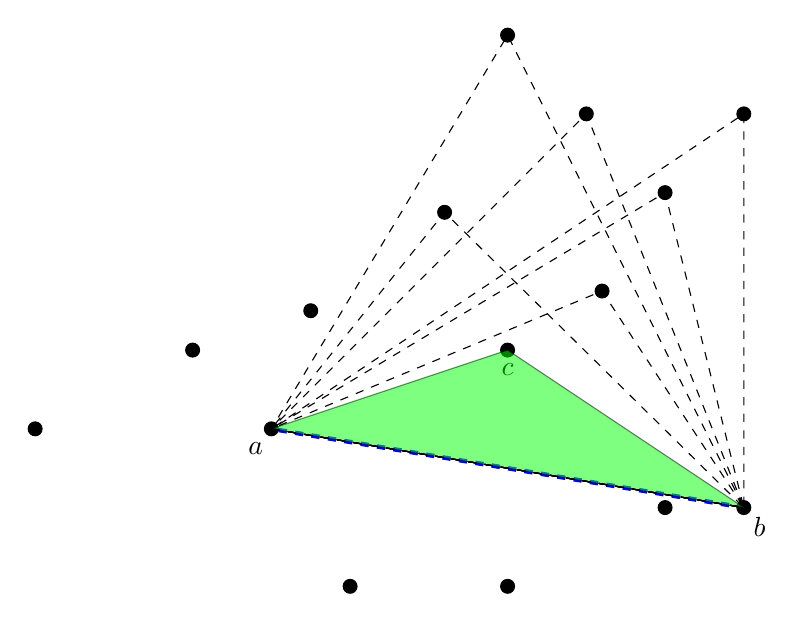
\begin{tikzpicture}
\node[draw, circle, black, fill=black, inner sep=0pt, minimum size=5pt] (h) at (0,0) {};
\node[draw, circle, black, fill=black, inner sep=0pt, minimum size=5pt] (c) at (2,3) {};
\node[] at (2, 2.75) {$c$};
\node[draw, circle, black, fill=black, inner sep=0pt, minimum size=5pt] (p) at (1.2,4.75) {};
\node[draw, circle, black, fill=black, inner sep=0pt, minimum size=5pt] (d) at (4,1) {};
\node[draw, circle, black, fill=black, inner sep=0pt, minimum size=5pt] (e) at (5,6) {};
\node[draw, circle, black, fill=black, inner sep=0pt, minimum size=5pt] (f) at (2,7) {};
\node[draw, circle, black, fill=black, inner sep=0pt, minimum size=5pt] (g) at (4,5) {};
\node[draw, circle, black, fill=black, inner sep=0pt, minimum size=5pt] (a) at (-1,2) {};
\node[] at (-1.2, 1.75) {$a$};
\node[draw, circle, black, fill=black, inner sep=0pt, minimum size=5pt] (i) at (-2,3) {};
\node[draw, circle, black, fill=black, inner sep=0pt, minimum size=5pt] (j) at (-0.5, 3.5) {};
% \node[draw, circle, black, fill=black, inner sep=0pt, minimum size=5pt] (k) at (2.5,-1) {};
\node[draw, circle, black, fill=black, inner sep=0pt, minimum size=5pt] (l) at (3,6) {};
\node[draw, circle, black, fill=black, inner sep=0pt, minimum size=5pt] (m) at (-4,2) {};
% \node[draw, circle, black, fill=black, inner sep=0pt, minimum size=5pt] (n) at (-2, -2) {};
\node[draw, circle, black, fill=black, inner sep=0pt, minimum size=5pt] (o) at (2, 0) {};

\node[draw, circle, black, fill=black, inner sep=0pt, minimum size=5pt] (b) at (5,1) {};
\node[] at (5.2, 0.75) {$b$};

\node[draw, circle, black, fill=black, inner sep=0pt, minimum size=5pt] (q) at (3.2, 3.75) {};

\draw[ultra thick, dashed, blue] (a) -- (b);
\draw[fill=green, opacity=0.5] (a.center) -- (b.center) -- (c.center) -- cycle;
\draw[dashed] (a.center) -- (b.center) -- (l.center) -- cycle;
\draw[dashed] (a.center) -- (b.center) -- (g.center) -- cycle;
\draw[dashed] (a.center) -- (b.center) -- (e.center) -- cycle;
\draw[dashed] (a.center) -- (b.center) -- (q.center) -- cycle;
\draw[dashed] (a.center) -- (b.center) -- (f.center) -- cycle;
\draw[dashed] (a.center) -- (b.center) -- (p.center) -- cycle;

\end{tikzpicture}
\caption{An illustration of the proof for~\Cref{thm:empty-triangle}.}
\label{fig:empty-triangle}
\end{figure}

Instead of formalizing the above proof, we will formalize a SAT-based proof, with the goal of approaching the formalization of the empty hexagon theorem.
Naturally, to use a  SAT-solver we need to parameterize~\Cref{thm:empty-triangle} by $n = |S|$, the number of points, and generate a different proof for each value of $n \geq 3$. For example, consider the following theorem.

\begin{lstlisting}
  theorem EmptyTriangle10Theorem (pts : Finset Point)
    (gp : PointFinsetInGenPos pts)
    (h : pts.card = 10) :
    ∃ (p q r : Point), {p, q, r} ⊆ pts ∧ EmptyTriangleIn p q r pts
\end{lstlisting}

To complete the statement of the theorem, we must define~\texttt{EmptyTriangleIn}, and before that what it means for a point to be \emph{inside} a triangle.

\begin{lstlisting}
  def pt_in_triangle (a : Point) (p q r : Point) : Prop :=
    ∃ p' q' r', ({p', q', r'} : Set Point) = {p, q, r} ∧
      Sorted₃ p' q' r' ∧
      Sorted₃ p' a r' ∧
      a ≠ q' ∧ -- this isn't needed if p,q,r are in GP
      σ p' q' r' = σ p' a r' ∧
      σ p' a q' = σ p' r' q' ∧
      σ q' a r' = σ q' p' r'

  /-- S is an empty triangle relative to pts -/
  structure EmptyTriangleIn (p q r : Point) (pts : Finset Point) : Prop :=
    gp : InGenPos₃ p q r
    empty: ∀ a ∈ pts, ¬(pt_in_triangle a p q r)
\end{lstlisting}


